\section{Methodology }
\label{ch6:sec:method}

\textit{DiffGeo} is designed to sample novel designs using a shape parameterization model and a function that maps a random normal distribution to the parameterization space.
To this end, we rely on the Latent Space Model (LSM)~\cite{aa.Wei2023,aa.Wei2023b} to provide an automatic shape parameterization represented by a learned latent space, denoted as $\bZ$.
Then we introduce the Latent Space Diffusion Model (LSDM, denoted as $g$), which progressively denoises a random normal vector into a valid latent code.

\subsection{Latent Space Geometry Parameterization}
For the latent representation, we employ the LSM to parameterize the design surface geometry. It relies on an auto-decoder design \cite{ai.Tan1995, ai.Park2019c} and is trained jointly with the latent space using a dataset of the collected shapes. This model maps a template shape $\hat{M}=\{\hat{V}, E\}$ with given $N$ vertices $\hat{V}=\{\bv_1, \bv_2,...,\bv_N\}$ and edges $E$, such as NACA-0012 for 2D airfoils or a mean shape in a more general case, conditioned on a $d$ dimensional latent vector $\bz$ that parameterizes the output geometry as
\begin{align}
    f_{\Theta} : \mathbb{R}^d \times \mathbb{R}^D \rightarrow \mathbb{R}^D \; , \label{ch6:eq:map_lsm} \\
    \mathbf{\delta v} = f_{\Theta}(\bz, \hat{\bv}) \; , \nonumber
\end{align} 
where $D\in {2,3}$ stands for the coordinate space dimensionality. 
LSM is a multi-layer perceptron (MLP) network and $\Theta$ represents the weights that control LSM $f$.
A deformed shape is obtained as $M=\{\hat{V} + f_{\Theta}(\bz, \hat{V}), E\}$. 

During training, we collect a dataset of $K$ surface geometries, denoted as $S_1,\ldots,S_K$, which only contains sampled surface points. The training objective is to optimize the weights $\Theta$ and the latent vectors that parameterize each training data $\textbf{z}_1,\ldots,\textbf{z}_K$. We write this as:
\begin{align}
  \Theta^*,\bZ^* 
    &=  \argmin_{\Theta,\bz_1,\ldots,\bz_K} \sum_{k=1}^K \cL_{LSM}(\hat{\bv} + f_{\Theta}(\bz_k, \hat{\bv}), S_k)
  \;+\;w_{\bz}\|\bz\|_2^2 \;,
\label{ch6:eq:argmin_f_z_theta}
\end{align}
where $\cL_{LSM}$ is a loss function that is minimized when $f_{\Theta}(\bz_k, \hat{\bv})$ yields a deformed airfoil geometrically identical to $S_k$. The optimal $\bz_k^*$ corresponds to a low-dimensional parameterization of $S_k$. We use the chamfer distance~\cite{ai.Barrow1977}, denoted as $\cL_{CD}(V, S)$, to measure the geometric difference.  Additionally, we apply a vector norm regularization on $\bz$ to ensure the smoothness of the acquired latent space. Therefore, the overall training objective becomes:
\begin{align}
  \cL_{LSM}(V, S) 
    &= \cL_{CD}(V, S) + w_{\bz}\left|\left|\bz\right|\right|^2 \nonumber \\
    &= \underbrace{\sum_{v\in V}\min_{s\in S}\left\|v - s\right\|_2^2\;+\;\sum_{s\in S}\min_{v\in V}\left\|s - v\right\|_2^2}_{\cL_{CD}(V,S)}  + w_{\bz}\left|\left|\bz\right|\right|^2 \; ,
\end{align}
where $w_{\bz}$ is the balancing weight.

At inference time, given a new target geometry $S$ and the frozen weights $\Theta^*$, the latent parameterization vector $\bz^*$ is obtained by finding
%
\begin{align}
  \bz^* &=  \argmin_{\bz} \cL_{LSM}(\hat{\bv} + f_{\Theta}(\bz, \hat{\bv}), S) \; .
\label{ch6:eq:agmin_f_z}
\end{align}
%
The output geometry becomes $M=\{\hat{V} + f_{\Theta}(\bz^*, \hat{V}), E\}$. 

To synthesize new geometries, we simply need to create new latent codes that fall within the distribution of plausible latent vector and then decode it into a deformed shape. However, it is intractable to directly sample from the distribution of $\bZ$, which is unknown and non-analytical. Therefore, we require the LSDM to sample from a feasible random distribution and project the sampled random vector to a valid latent vector.

\subsection{Latent Space Diffusion Model for Unconditional Generation}

\begin{figure}[!t]
    \begin{center}
        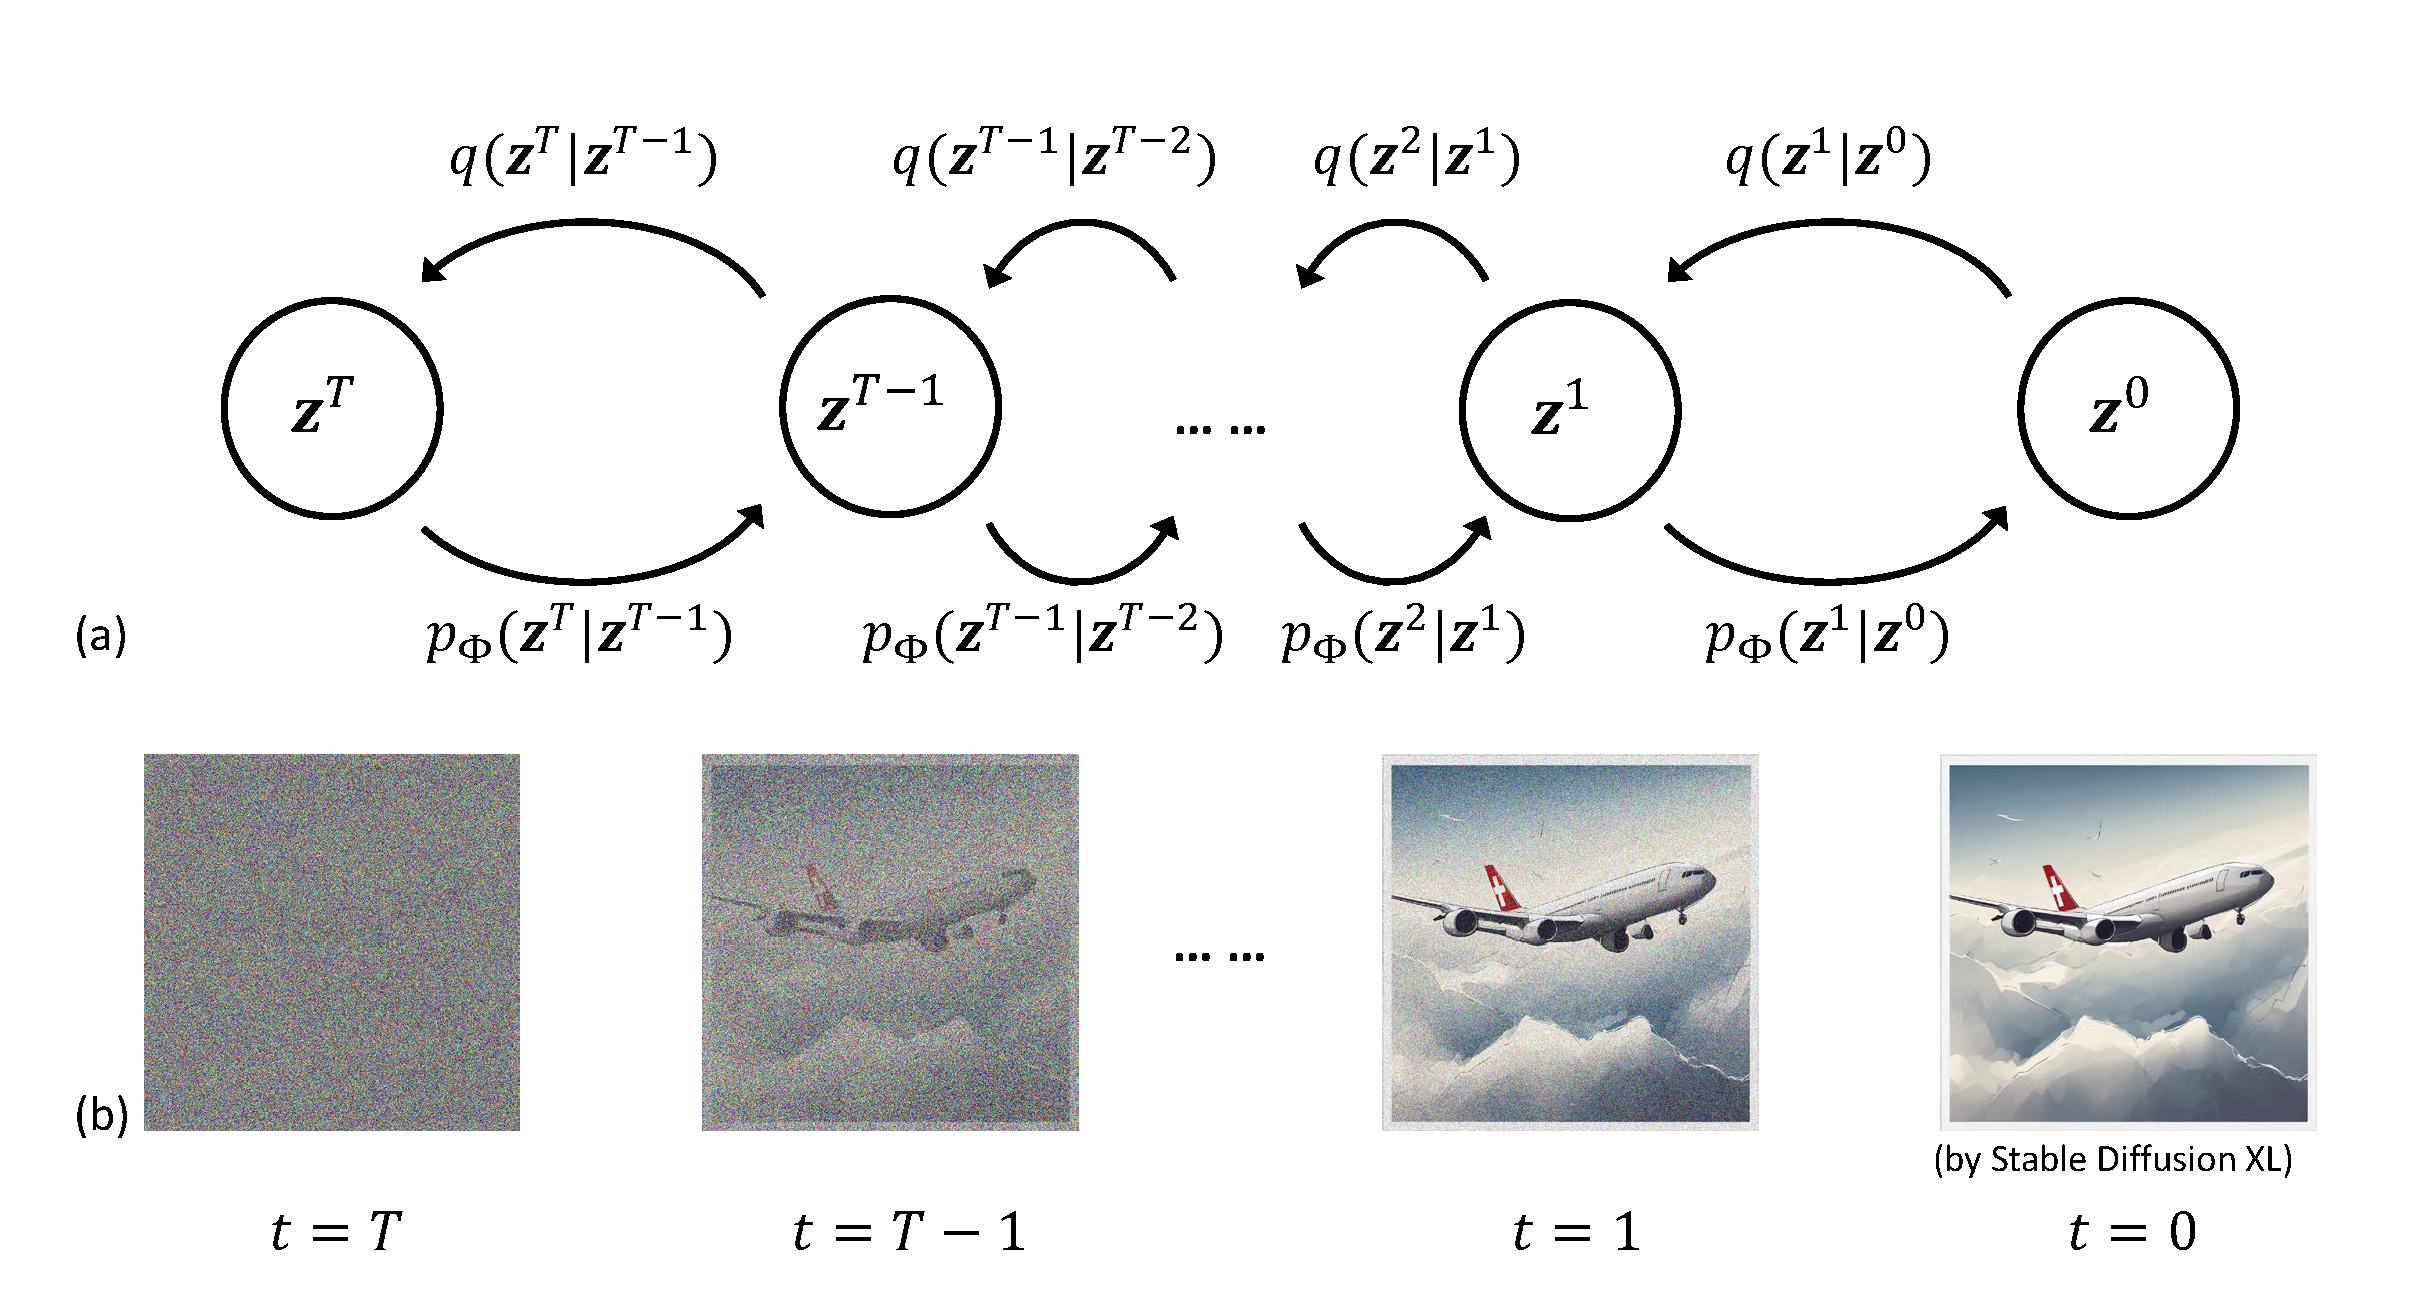
\includegraphics[width=0.95\linewidth]{chapter6/fig/ddpm.pdf}
    \end{center}
    \vspace{-4mm}
    \caption{
        \small LSDM's forward and reverse processes represented in (a) latent-space Markov chain, (b) an analogy on image diffusion.
    }
    \label{ch6:fig:abs_ddpm}
\end{figure}

The LSDM is a probabilistic generative model that maps a standard multivariate normal distribution to the latent space of the LSM via a Markov chain parameterization. It follows the denoising diffusion probabilistic model (DDPM) framework~\cite{ai.Ho2020}, which defines a forward noising process $q$, and a learned reverse process $p_\Phi$, as shown in Fig.~\ref{ch6:fig:abs_ddpm}(a). For clarity, Fig.\ref{ch6:fig:abs_ddpm}(b) illustrates an analogous image-based diffusion process.

In the forward process, Gaussian noise is added with variance schedules $\{\beta_t\}^T_{t=1}$, $\alpha_t=1-\beta_t$ and $\bar{\alpha}_t=\Pi^t_{s=1}\alpha_s$. The noisy latent vector at step $t$ can be efficiently sampled in closed form as:
\begin{equation}
    q(\bz^t | \bz^0) = \cN(\bz^t; \sqrt{\Bar{\alpha}_t} \bz^0, (1-\Bar{\alpha}_t) \bI)\;.
\end{equation}
The reverse process starts from $p(\bz^T)=\cN(\bz^T; \textbf{0}, \bI)$ and uses Gaussian transitions $p_\phi(\bz^{t-1} | \bz^t) := \cN(\bz^{t-1}: \bmu_\phi(\bz^t, t), \beta_t \bI)$, where the mean is parameterized in the noise-prediction form:
\begin{equation}
    \bmu_\phi(\bz^t, t) := \frac{1}{\sqrt{\alpha_t}} (\bz^t - \frac{1-\alpha_t}{\sqrt{1-\Bar{\alpha}_t}}) g_\Phi(\bz^t, t)\;,
\end{equation}
where $g_\Phi(\bz^t, t)$ is the LSDM network based on the Multi-Layer Perceptron (MLP) structure.

The network is trained with the standard noise-matching loss:
\begin{equation}
    \cL_{LSDM} := \mathbb{E}_{t, \bz^0, \mathbf{\epsilon}\sim \cN(\textbf{0}, \bI)} 
    \left[ \left| \left|
    \mathbf{\epsilon} - g_\Phi \left(\sqrt{\Bar{\alpha}_t} \bz^0 + \sqrt{1-\Bar{\alpha}_t}\mathbf{\epsilon}, t \right)
    \right|\right| ^ 2\right]\;,
\end{equation}
with training steps summarized in Algorithm~\ref{ch6:alg:abs_train_diffusion}.
\begin{algorithm}
    \caption{The training steps of the diffusion network in LSDM.}
    \label{ch6:alg:abs_train_diffusion}
    \begin{algorithmic}
        \While {not converged}
            \State sample a latent code from the training dataset as $\bz^0$.
            \State $t \sim \text{Uniform}(\{1,2,...,T\})$ 
            \State $\mathbf{\epsilon} \sim \cN(\mathbf{0}, \bI)$
            \State Take gradient descent optimization step on $\nabla_\Phi \left|\left| \mathbf{\epsilon} - g_\Phi \left(\sqrt{\Bar{\alpha}_t} \bz^0 + \sqrt{1-\Bar{\alpha}_t}\mathbf{\epsilon}, t \right) \right|\right|^2$.
        \EndWhile
    \end{algorithmic}
\end{algorithm}

From the score-matching theory~\cite{ai.Song2021c}, the trained $g_\Phi$ estimates the score function of the reverse process: 
\begin{equation}
    \nabla_{\bz^t} \log p_\Phi(\bz^t|\bz^{t+1})=-\frac{1}{\sqrt{1-\Bar{\alpha}_t}}  g_\Phi(\bz^t, t) \;.
\end{equation}
Unconditional sampling starts from $\bz^t\sim \cN(\textbf{0}, \bI)$ and iteratively applies the reverse transition (summarized in Algorithm~\ref{ch6:alg:abs_sample_diffusion}) with the stochastic gradient Langevin dynamics~\cite{ai.Welling2011} until $\bz^0$ is obtained and decoded to a shape.

\begin{algorithm}
    \caption{The unconditional sampling steps of LSDM.}
    \label{ch6:alg:abs_sample_diffusion}
    \begin{algorithmic}
        \State $\bz^T \sim \cN(\mathbf{0}, \bI)$
        \For{$t=T,T-1,...,1$}
            \State $\mathbf{\epsilon} \sim \cN(\mathbf{0}, \bI)\;\text{if } t>1\;\text{, else } \mathbf{\epsilon}=0$ 
            \State $\bz^{t-1} = \frac{1}{\sqrt{\Bar{\alpha}_t}} \left(\bz^t - \frac{1-\alpha_t}{\sqrt{1-\Bar{\alpha}_t}} g_\Phi(\bz^t, t) \right) + \sqrt{\beta_t}\mathbf{\epsilon}$
        \EndFor 
        \State \textbf{return} {$\bz^0$}
    \end{algorithmic}
\end{algorithm}

\subsection{Conditional Latent Space Diffusion Model}
When developing generative models for aerospace engineering design, the sampling should be biased toward regions that satisfy design objectives and constraints. Formally, this amounts to solving
\begin{align}
    & \min_{V} O(V) \; , \nonumber\\
    \text{subject to} \quad & C^E_i(V) = 0 \;\; (i=1,\dots,m) \; , \\
    & C^I_j(V) \le 0 \;\; (j=1,\dots,r) \; , \nonumber
\end{align}
where $O$ denotes the primary objective, $C^E_i$ are equality constraints and $C^I_j$ are inequality constraints. 
%
To impose these constraints during generation, we define an energy function that quantifies constraint satisfaction as a differentiable scalar loss. This energy function takes the form of a penalty:
\begin{equation}
    E(V)=\bigl\|O(V)\bigr\|^2 + \sum_{i=1}^m \rho_i \bigl\|C^E_i(V)\bigr\|^2 + \sum_{j=1}^r \gamma_j \bigl\|\max(0,C^I_j(V))\bigr\|^2 \quad ,
    \label{ch6:eq:energy_guidance}
\end{equation}
where $\rho_i > 0, \gamma_j > 0$ are penalty coefficients weighting the violation of equality and inequality constraints, respectively.

We incorporate this energy function into the sampling process as a guiding signal and formulate the conditional latent-space diffusion model (CLSDM). At each reverse diffusion step $t$, the energy is evaluated based on the current latent code $\bz^t$ and the decoded geometry $V^t=\hat{V}+f_\Theta(\bz^t)$. For simplicity, we denote: $E(\bz^t):=E(f_\Theta(\bz^t))=E(V^t)$.

To bias the sampling toward low-energy geometries, we define an unnormalized energy-augmented distribution over $\bz^t$, which we write as:
\begin{equation}
    \hat{p}_\Phi(\bz^t) \propto p_\Phi(\bz^t)e^{-\xi E(\bz^t)},
\end{equation}
where $\xi>0$ is a temperature parameter controlling the strength of guidance. At the sampling timestep $t$, The adjusted score function under this distribution becomes:
\begin{equation}
    \nabla_{\bz^t} \log \hat{p}_\Phi(\bz^t|\bz^{t+1})=-\frac{1}{\sqrt{1-\Bar{\alpha}_t}}  g_\Phi(\bz^t, t) - \xi\nabla_{\bz^t}E(\bz^t)\;.
\end{equation}

This modification augments the original score function of reversed process with a gradient that encourages geometries satisfying the design objectives. The full conditional sampling procedure is outlined in Algorithm~\ref{ch6:alg:abs_sample_conditional_diffusion}.
\begin{algorithm}
    \caption{The conditional sampling steps of CLSDM.}
    \label{ch6:alg:abs_sample_conditional_diffusion}
    \begin{algorithmic}
        \State Given: generation target in differentiable forms of $O,C^E,C^I$.
        \State $\bz^T \sim \cN(\mathbf{0}, \bI)$
        \For{$t=T,T-1,...,1$}
            \State $\mathbf{\epsilon} \sim \cN(\mathbf{0}, \bI)\;\text{if } t>1\;\text{, else } \mathbf{\epsilon} \text{ is all zero}$ 
            \State Compute $E(\bz^t)$,
            \State $\bz^{t-1} = 
                \frac{1}{\sqrt{\Bar{\alpha}_t}} 
                \left( 
                    \bz^t - 
                    \frac{1-\alpha_t}{\sqrt{1-\Bar{\alpha}_t}} g_\Phi(\bz^t, t) - 
                    \xi\nabla_{\bz^t} E(\bz^t) 
                \right) 
                + \sqrt{\beta_t}\mathbf{\epsilon}$
        \EndFor 
        \State \textbf{return} {$\bz^0$}
    \end{algorithmic}
\end{algorithm}

When the energy function encodes complex design objectives or tight constraints, especially in 3D shape generation, the two goals of sampling from the learned distribution and minimizing the energy function may not align perfectly in convergence speed within the fixed number of diffusion steps $T$. As a result, the final samples may not fully satisfy the design criteria.

To address this issue, we propose an enhanced conditional sampling strategy for CLSDM that extends Algorithm~\ref{ch6:alg:abs_sample_conditional_diffusion}. After the initial generation, if the decoded geometry fails to meet the desired objectives, we partially reintroduce noise to the latent vector by simulating a forward diffusion process up to an intermediate noise level $T^*$, where $1<T*<T$. The reverse diffusion is then restarted from this noisy latent vector. This re-noising and re-generation loop is repeated for a fixed number of iterations, allowing the model to explore alternative paths while remaining near the solution manifold. The complete procedure of enhanced conditional sampling is summarized in Algorithm~\ref{ch6:alg:abs_sample_enhanced_conditional_diffusion}.

\begin{algorithm}
    \caption{The enhanced conditional sampling steps of CLSDM.}
    \label{ch6:alg:abs_sample_enhanced_conditional_diffusion}
    \begin{algorithmic}
        \State Given: generation target in differentiable forms of $O,C^E,C^I$;
        \State \qquad\quad number of enhanced loops $N_{T^*}$;
        \State \qquad\quad noising level $T^*$.
        \State $\bz^T \sim \cN(\mathbf{0}, \bI)$
        \For{$t=T,T-1,...,1$}
            \State $\mathbf{\epsilon} \sim \cN(\mathbf{0}, \bI)\;\text{if } t>1\;\text{, else } \mathbf{\epsilon}\text{ is all zero}$ 
            \State Compute $E(\bz^t)$,
            \State $\bz^{t-1} = 
                \frac{1}{\sqrt{\Bar{\alpha}_t}} 
                \left( 
                    \bz^t - 
                    \frac{1-\alpha_t}{\sqrt{1-\Bar{\alpha}_t}} g_\Phi(\bz^t, t) - 
                    \xi\nabla_{\bz^t} E(\bz^t) 
                \right) 
                + \sqrt{\beta_t}\mathbf{\epsilon}$
        \EndFor 
        \For{$n=1,2,...,N_{T^*}$}
            \State $\mathbf{\tau} \sim \cN(\mathbf{0}, \bI)$
            \State $\bz^{T^*} = \sqrt{\Bar{\alpha}_{T^*}} \bz^0 + \sqrt{1-\Bar{\alpha}_{T^*}}\mathbf{\tau}$
            \For{$t=T^*,T^*-1,...,1$}
                \State $\mathbf{\epsilon} \sim \cN(\mathbf{0}, \bI)\;\text{if } t>1\;\text{, else } \mathbf{\epsilon}=0$ 
                \State Compute $E(\bz^t)$,
                \State $\bz^{t-1} = 
                    \frac{1}{\sqrt{\Bar{\alpha}_t}} 
                    \left( 
                        \bz^t - 
                        \frac{1-\alpha_t}{\sqrt{1-\Bar{\alpha}_t}} g_\Phi(\bz^t, t) - 
                        \xi\nabla_{\bz^t} E(\bz^t) 
                    \right) 
                    + \sqrt{\beta_t}\mathbf{\epsilon}$
            \EndFor
        \EndFor
        \State \textbf{return} {$\bz^0$}
    \end{algorithmic}
\end{algorithm}

\subsection{Implementation Details}
Both LSM and LSDM are implemented using the PyTorch~\footnote{pytorch.org} toolbox and are capable of GPU acceleration. The dimension of LSM's latent space is $d=256$. We use the Adam optimizer~\cite{ai.Kingma2015b} with the learning rate of $5\times10^{-4}$ for LSM's weights $\Theta$ and $10^{-3}$ for the latent space $\bZ$.

LSDM is implemented as an MLP model and it has three hidden layers and leaky ReLU activation functions. The forward and reverse processes use $T=1000$ time steps. The diffusion scheduler $\beta$ linearly increases from $10^{-4}$ to $0.02$ as $t$ ranges from $0$ to $T$, and remains constant in both forward and reverse processes. The LSDM is trained with the AdamW optimizer~\cite{ai.Loshchilov2019} and a learning rate of $10^{-5}$. Under these implementation settings, \textit{DiffGeo} is computationally efficient. For example, when developing the 2D airfoil generator, the training of LSM and LSDM with a dataset of 50 airfoils take $671.9$ seconds and $716.4$ seconds on an NVIDIA V100 graphics card, respectively.
The averaged time cost of unconditional airfoil generation is $690.51$ milliseconds per 50 samples.